\subsection{Eure Profs}
Um euch einen kleinen Vorgeschmack auf die Leute zu geben, die euch
demn"achst mit ihrem Wissen begl"ucken wollen, seien hier einige
aufgeführt. 
% Für n-te SS
%Einige davon werdet ihr allerdings erst in höheren Semestern zu Gesicht
%bekommen.

%%Die Vorlesung wird jedes Jahr im Sommersemester angeboten.

%Programmiert wird hier fast ausschlie"slich in Java. Wer keine oder nur wenig Erfahrungen mit Java gemacht hat, sollte unbedingt die kleinen "Ubungen bearbeiten.
%\newpage
\subsubsection{Einführung in die Logik}%ier geht
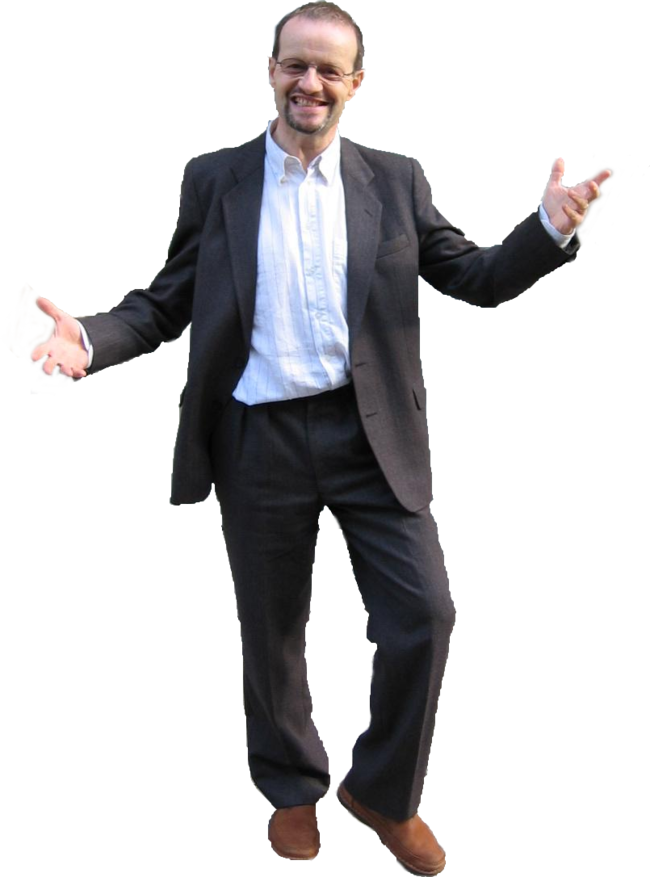
\includegraphics[width=0.8\linewidth]{bilder/dozenten/adamek.png}\\
\textit{Prof.  Adámek}\\
Die Vorlesung behandelt die Grundlagen der formalen Logik, mit einen
starken Fokus auf Aussagen- und Prädikatenlogik. Die Hausaufgaben sind
dabei teilweise sehr zeitaufwändig, aber dafür eine gute
Klausurvorbereitung. Dabei ist das Skript sehr hilfreich.
\\
\subsubsection{Analysis für Informatiker}

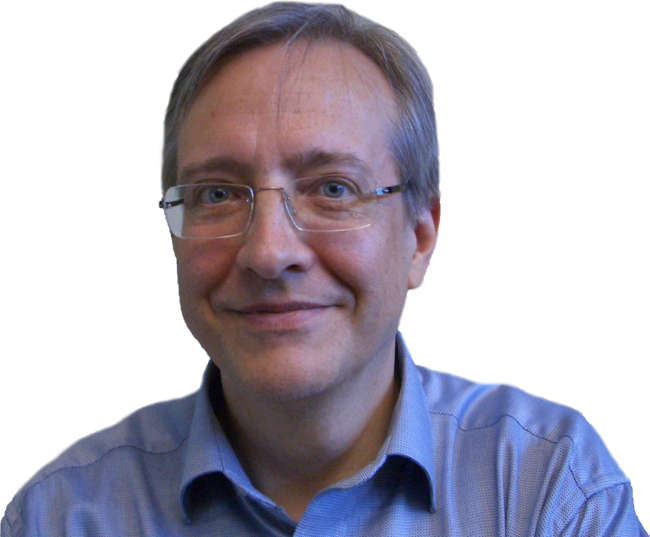
\includegraphics[width=0.8\linewidth]{bilder/dozenten/marten_frei.png}\\
\textit{Dr. Wolfgang Marten}\\

Hier geht es um Differential- und Integralrechnung, sowie Grenzwerte. %Gruppentheorie.
Die "Ubungen sind zwar nicht immer einfach, geben aber einen sehr guten Ausblick auf die Klausur.
\subsubsection{Computernetze 1}

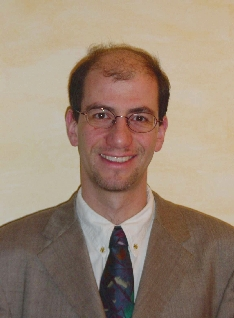
\includegraphics[width=0.8\linewidth]{bilder/dozenten/wolf}\\
\textit{Prof. Lars Wolf}\\
Hier lernt man die grundlegende Funktionsweise von Netzwerken
kennen. Für die Klausur sollte man auf gar keinen Fall die Übungen
verpassen. Interessiert man sich über die Vorlesung hinaus fürs Thema,
kann man sich einen Tanenbaum aus der Uni-Bibliothek besorgen.
\footnote{Nein, dort gibt es - vorallem um diese Jahreszeit - keinen 
Verleih für weihnachtliche Dekoration mit Rechtschreibdefiziten. 
Gemeint ist hier \textit{Computernetzwerke}, eines der fünf 
beliebten Lehrücher von Andrew S. Tanenbaum.}

\subsubsection{Wissenschaftliches Arbeiten}

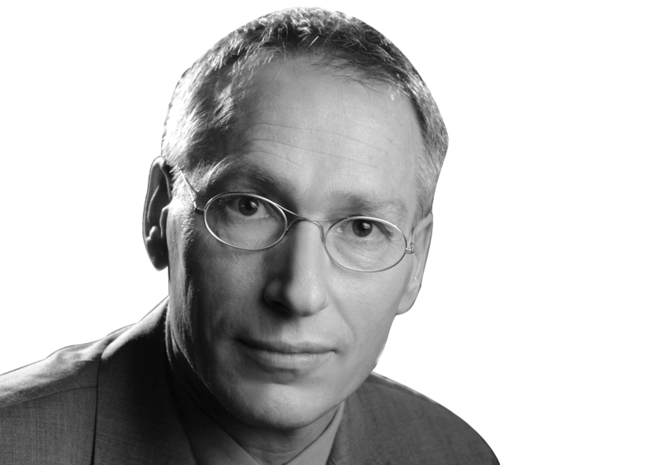
\includegraphics[width=0.9\linewidth]{bilder/dozenten/jung_frei.png}\\
\textit{Prof. Helmut Jung}

In dem Kurs "`wissenschaftliches Arbeiten"' lernen die Teilnehmer/-innen, Schritt f"ur Schritt eine wissenschaftliche Arbeit durchzuf"uhren -- beispielsweise eine Bachelorarbeit.
Hierzu erfahrt ihr, wie man systematisch vorgeht und welche Methoden
man in welchem Schritt verwenden kann. Er ist eine freiwillige
Schlüsselqualifikation, die Teilnahme wird aber empfohlen.

% \subsubsection{Algorithmen und Datenstrukturen}
% 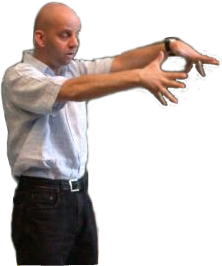
\includegraphics[width=0.7\linewidth]{bilder/dozenten/fekete_frei.png}\\
% \textit{Prof. S\'andor Fekete}\\

% Diese Vorlesung vermittelt Programmiersprachenunabh"angige Konzepte wie B"aume, Listen oder Stacks. Wer nicht wei"s, was sich hinter diesen Begriffen verbirgt, sollte auf keinen Fall die "Ubungen verpassen.
% Sie findet jedes Jahr im WS statt.

\subsubsection{Programmieren 1/Programieren 2}
 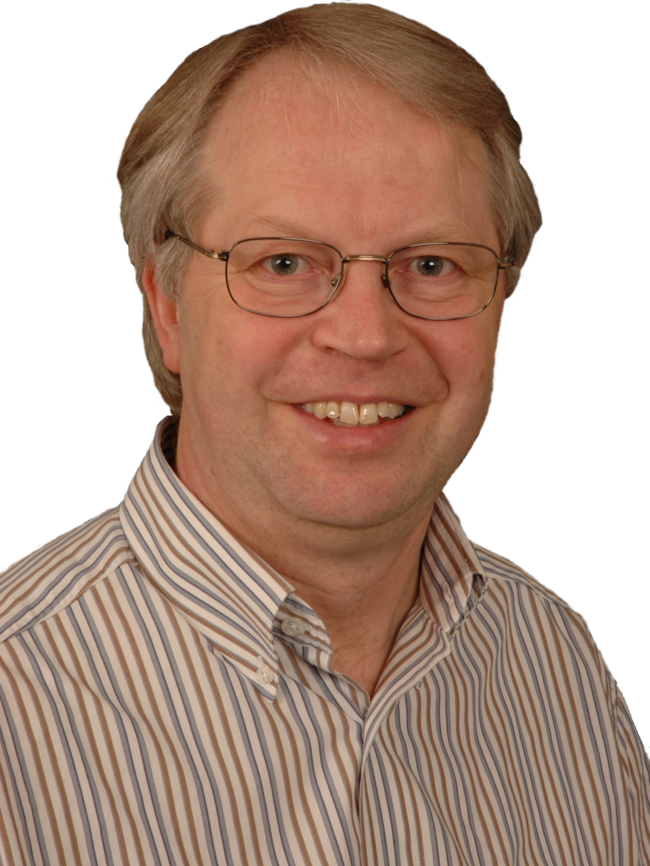
\includegraphics[width=0.6\linewidth]{bilder/dozenten/struck.png}\\
\textit{Dr. Werner Struckmann}\\
%Programmiert wird hier fast ausschlie"slich in Java.
%Die Vorlesungen werden im Jahresturnus angeboten, wobei 
%Programmieren 1 
%im WS, Programmieren 2 hingegen im SS angeboten wird. 
%Dabei geht es im 1.
In ,,Programmieren 1'' (jährlich Wintersemester) geht es um grundlegende Konzepte der Programmierung am Beispiel von
Java.  Darauf aufbauend wird in ,,Programmieren 2'' (jährlich Sommersemester) die 
die Implementierung von Algorithmen und Datenstrukturen geübt. 
%Wer keine oder nur wenig Erfahrungen mit Java gemacht hat, sollte unbedingt die kleinen "Ubungen bearbeiten.
Hat man  schon Vorkenntnisse in einer Programmiersprache (etwa
durch eine Ausbildung zum Fachinformatiker o.Ä.) kann man sich
durchaus auch schon im 1. Semester an Programmieren 2 versuchen, die
Reihenfolge ist NICHT vorgeschrieben. 
%\subsubsection{Diskrete Mathematik}

% \begin{figure}[h]
% 	\centering\includegraphics[width=0.7\linewidth]{bilder/kemnitz.png}\\
% 	{Dr. Arnfried Kemnitz}
% \end{figure}
%Diskrete Mathematik handelt von allem, was mit ganzen Zahlen zu tun hat: Fibbonacci-Zahlen, Primzahlen, Modulorechnung, usw.
%Die Veranstaltung wird von Prof. Arnfried Kemnitz jährlich im WS
%gehalten (leider kein Foto). Ähnlich wie bei Analysis


%Die Klausur ist ber"uhmt f"ur ihre hohe Durchfallquote! (Gl"ucklicherweise sind daran nicht die Informatiker schuld)
%Trotzdem: Programmieren ist das Handwerk der Informatik, also macht eurem Fach Ehre.

%Die Veranstaltung findet in zwei Gruppen statt, eine bei Prof. Jung und die andere bei Dr. Herrmann.
% Das gehört eigentlich nicht hier hin:

%Die Veranstaltung wird in zwei Gruppen angeboten: Der erste Kurs bei Prof. Jung findet Montag von 9:45 bis 11:15 Uhr und Dienstag von 11:30 bis 14:45 Uhr statt.
%Der zweite Kurs bei Dr. Herrmann findet Dienstag von 15:00 bis 16:30 Uhr statt.
%Beide Kurs haben denselben Inhalt und dieselbe Stundenzahl.
%Der zweite Kurs dauert das gesamte Semester, der andere endet entsprechend fr"uher.

%%% Local Variables: 
%%% mode: latex
%%% TeX-master: "../../1-te"
%%% End: 
